\section{Results}
\label{sec:results}


\begin{figure}
  % Requires \usepackage{graphicx}
  \begin{center}
	\begin{tabular}{ccc}
	  \parbox{40mm}{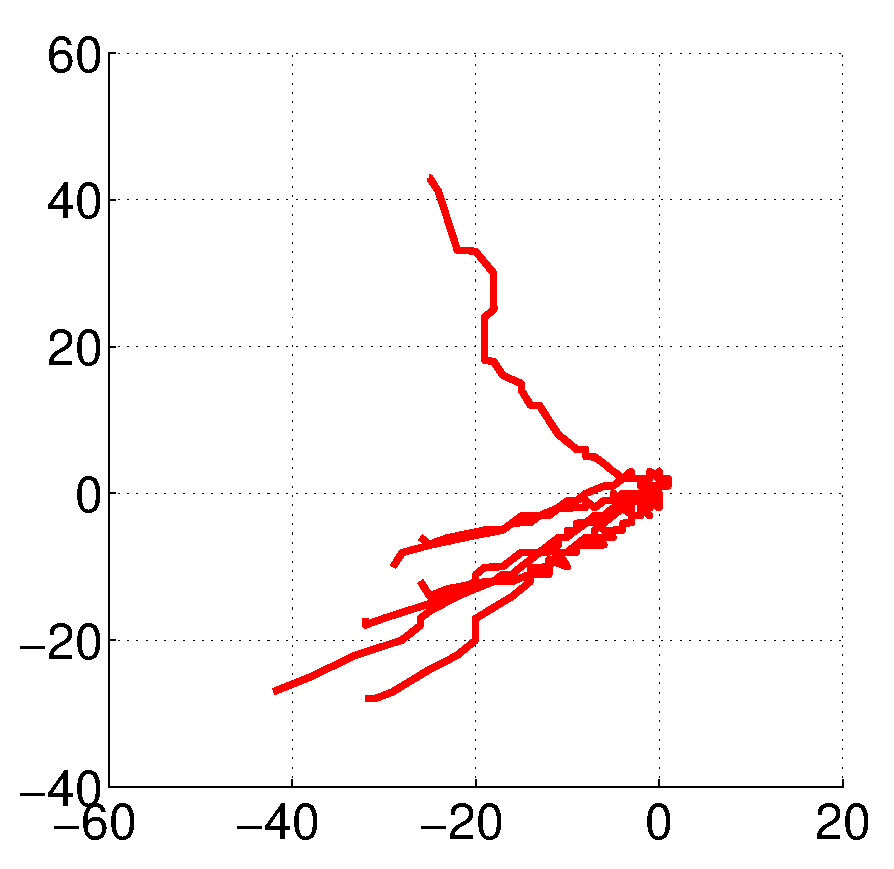
\includegraphics[width=40mm]{Figure/LeftEyeClosedLoop.eps}}  & \hspace{2cm} &
	  \parbox{40mm}{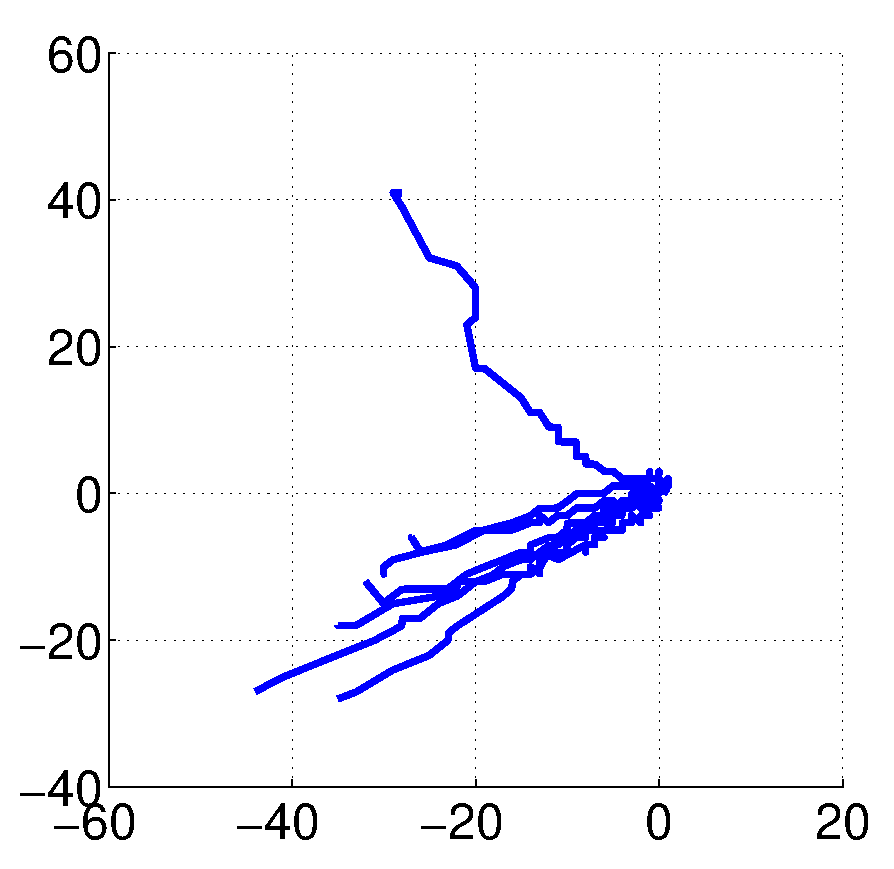
\includegraphics[width=40mm]{Figure/RightEyeClosedLoop.eps}}
	  \\
	  Left eye & \hspace{2cm} & Right eye
	  %	  \end{t\\
	  %	Top view & & Lateral view
  \end{tabular}
\end{center}
\caption{The left picture shows a top view of the eyeball and indicates the version (top) and the vergence (down) angles. The right picture instead shows the lateral view with the common (top) and differential tilt (down) angles.}\label{Fig:ImagePlaneClosedLoopErrors}
  \end{figure}

\begin{figure}
  % Requires \usepackage{graphicx}
  \begin{center}
	\begin{tabular}{ccc}
	  \parbox{40mm}{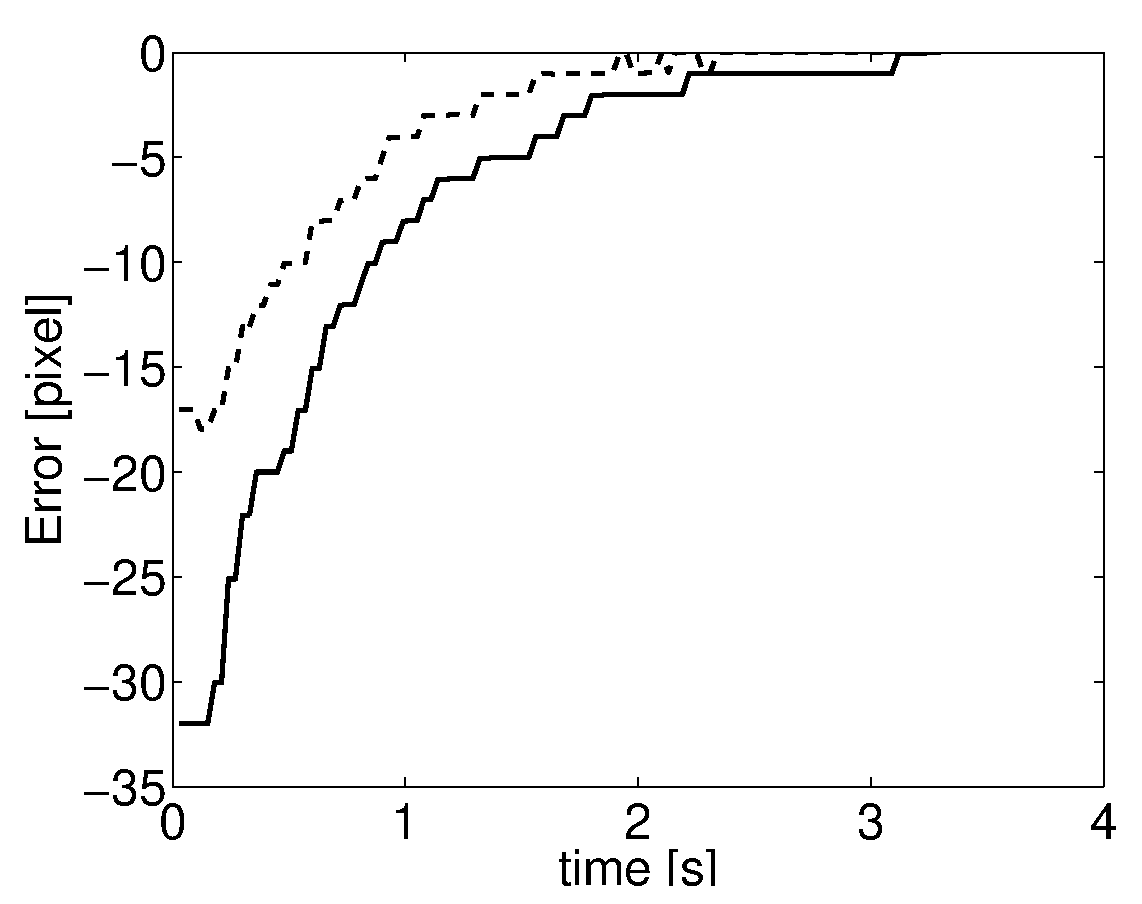
\includegraphics[width=40mm]{Figure/TimeReponseLeftClosedLoop.eps}}  & \hspace{2cm} &
	  \parbox{40mm}{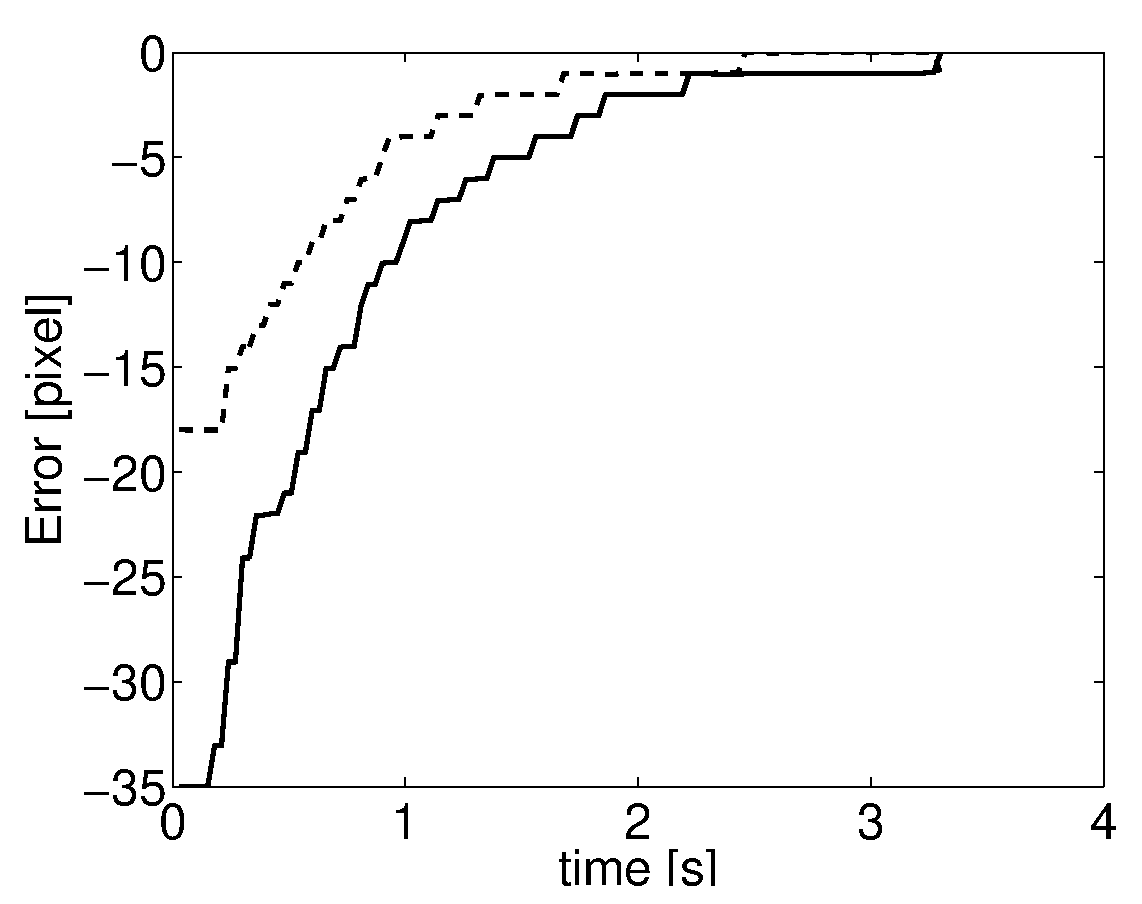
\includegraphics[width=40mm]{Figure/TimeReponseRightClosedLoop.eps}}
	  \\
	  Left eye & \hspace{2cm} & Right eye
	  %	  \end{t\\
	  %	Top view & & Lateral view
  \end{tabular}
\end{center}
\caption{The left picture shows a top view of the eyeball and indicates the version (top) and the vergence (down) angles. The right picture instead shows the lateral view with the common (top) and differential tilt (down) angles.}\label{Fig:TimeResponseClosedLoopErrors}
  \end{figure}
